\chapter{Design}
	
	After the security audit, it was apparent that the majority of the codebase needed to be refactored in order to make it object-oriented.
	The decision to rewrite the program was not a light one, by rewriting the program, the scope of extensions to \ac{AWESOME} became much more limited via time constraints.
	
	With the rewrite came the opportunity to utilise both a framework and a design pattern.
	Frameworks were ruled out under the stance that it had to be deployed on a server without shell access.
	However later research discovered that this is achievable in Laravel\footnote{Laravel Homepage: \url{http://laravel.com}}, which would have been the framework of choice for several reasons.
	
	Laravel would have provided a complete, and mature \ac{MVC} framework, as well as an \ac{i18n} framework and a solid basis for \ac{AWESOME}.
	Ultimately, poor research into Laravel on a shell-less server resulted in an attempt to produce a bespoke \ac{MVC} framework, which, unsurprisingly is harder than it first seems.
	
	\section{Programming Language}
	
	The programming language choice was fairly fixed, as it had to be easily runnable on an \ac{AU} server.
	This limited the choice to PHP, but which minor version of PHP was only found out later in the project which is discussed further in \autoref{sec:implementation}.
	
	If this requirement wasn't an issue, Ruby on Rails would have been the ideal candidate for this project, as it already provides an \ac{MVC} framework and gems for \ac{i18n}.
	
	\section{\acl{MVC} Framework}
	
	Since using a framework was ruled out, a custom-made \ac{MVC} framework was written to support this project.
	The design of which is laid out in this section and is very heavily taken from the `Write your own PHP MVC Framework' series of tutorials\cite{php-mvc-tutorial}.
	
	\subsection{Routing}
	
	URL Routing is a way to access specific controllers and views from a URL.
	This works via an Apache rewrite rule, which appends a \$\_GET variable which contains the current requested URL.
	
	\subsection{Directory Structure}
	
	\autoref{fig:mvcdirtree} shows the directory structure of the \ac{MVC} framework. `\textit{src}' is the source code to the program. Inside it contains everything needed to run \ac{AWESOME}.
	Inside `\textit{tests}' are the unit tests to be run automatically by TravisCI and PHPUnit.
	
	`\textit{src/app}' has the MVC classes which are used when the routing engine rewrites URLs.
	`\textit{src/config}' contains the config file for the program.
	In this file, database credentials are set, as well as SMTP mail server settings, some \ac{i18n} settings, and the debug flag which displays errors and shows a feedback form/notice (See \autoref{fig:feedbackform}).
	
	`\textit{src/db}' is a directory for \ac{SQL} dumps for the database schema.
	`\textit{src/i18n}' contains translation files for the \ac{i18n} framework, but more detail is in \autoref{sec:i18nframework}
	
	`\textit{src/lib}' is the `glue' that holds the MVC framework together.
	It contains the autoloader class, the bootstrap script and the third-party, open source PHPMailer\cite{phpmailer} classes used for sending mail via SMTP.
	
	`\textit{src/logs}' is where any PHP errors get logged when debug mode is off. This is in order to hide any potential security issues with displaying errors.
	
	`\textit{src/public}' is the main entry point to the program and where the Apache vhost will be set.
	`\textit{src/public/assets}' contains the Javascript, SASS, CSS, and images used in the HTML.
	Users with a valid token will be taken to their corresponding questionnaire.
	`\textit{src/public/admin}' is protected by HTTP authentication to prevent anybody from creating surveys and sending them out, or reading the results of previous surveys.
	
	\begin{figure}[H]
		\dirtree{%
			.1 AWESOME.
			.2 src.
			.3 app.
			.4 controllers.
			.4 models.
			.4 views.
			.3 config.
			.3 db.
			.3 i18n.
			.3 lib.
			.3 logs.
			.3 public.
			.4 admin.
			.4 assets.
			.2 tests.
		}
		\caption{Directory structure of the \acs{MVC} Framework}
		\label{fig:mvcdirtree}
	\end{figure}	
	
	\section{Internationalisation Framework}
	\label{sec:i18nframework}
	
	The \ac{i18n} framework is a standalone \ac{OOP} module which utilises JSON formatted files with strings for translation.
	
	\section{Database Schema}
	
	The database schema (see \autoref{fig:schema}) used is very similar to the prototype version.
	Documentation needed to be written for the existing schema, so the opportunity was taken to make some changes in the structure of the database before this happened.
	The old database schema did not use any foreign key constraints, nor was the use of primary keys ideal.
	
	Foreign keys are very useful to have in a system like this, as orphaned rows can be cleaned up nicely with a cascade delete.
	This prevents any data remaining in the table incase it is missed by an \ac{SQL} query that hasn't been updated in the code.
	
	I also made some changes to the way things were named, mostly to prevent confusion.
	In the new schema, a survey is a set of questionnaires, each of which is tailored to a specific student.
	In the old schema, everything was called a questionnaire, which led to confusion between a group of questionnaires and a single questionnaire.

	Additional changes need to be made in order for \ac{AWESOME} to support multiple departments across the university, but this is out of the scope of the dissertation, although this feature is on the roadmap if \ac{AWESOME} is to be used university-wide.
	
	\begin{figure}[H]
		\hspace{-0.165\textwidth}
		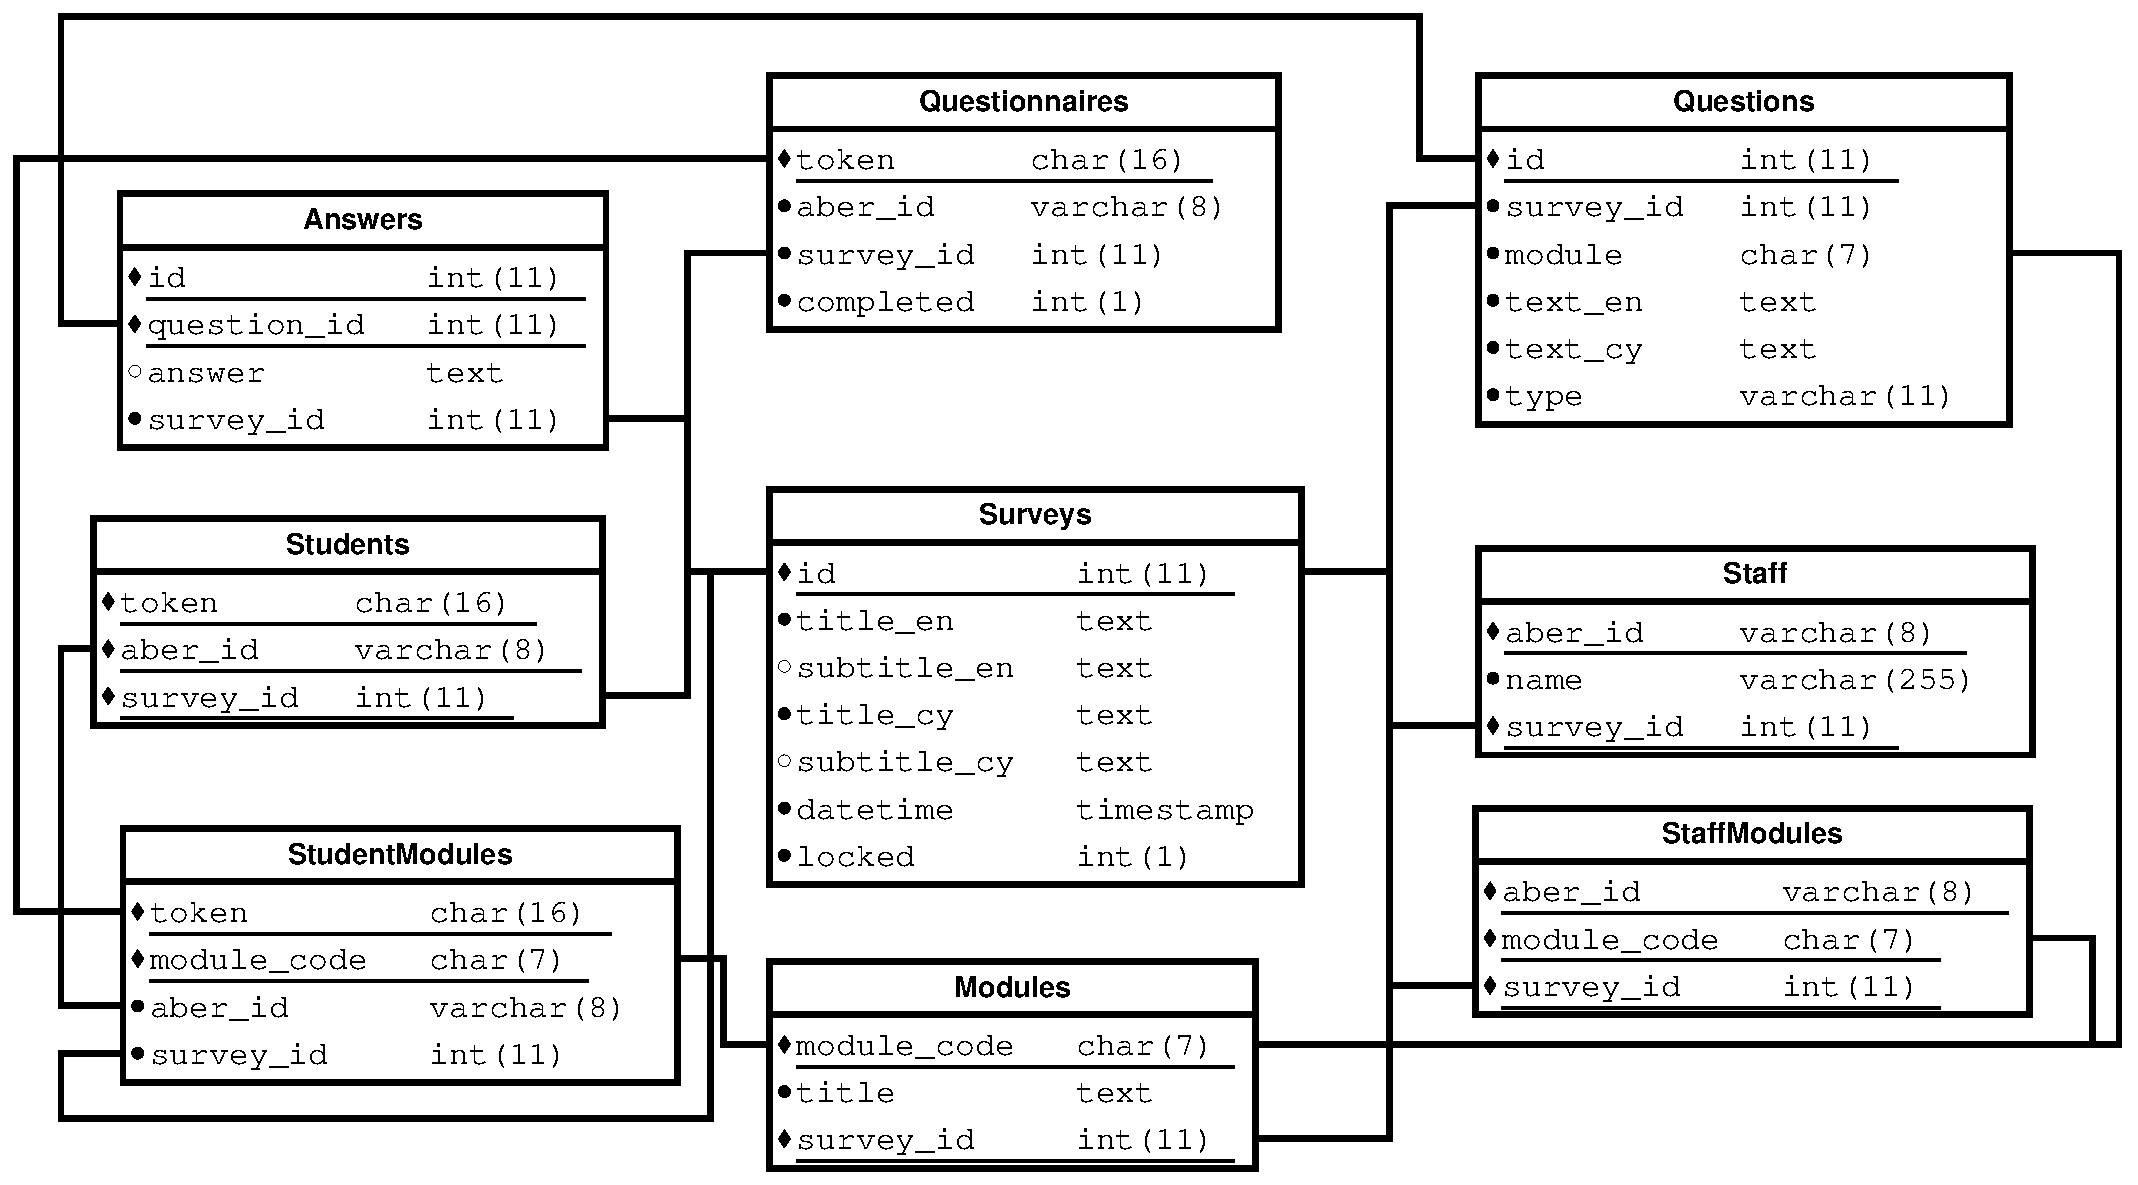
\includegraphics[width=1.33\textwidth]{schema}
		\caption{\ac{AWESOME} database schema design.}
		\label{fig:schema}
	\end{figure}
	
	\section{User Interface}
	
	The user interface was fairly good on the questionnaire-side in the prototype, so a lot of elements were re-used in that, with a few minor changes.
	
	\autoref{fig:questionnaire-comparison} shows a comparison between the prototype version and the submitted version of \ac{AWESOME}.
	
	\begin{figure}[H]
		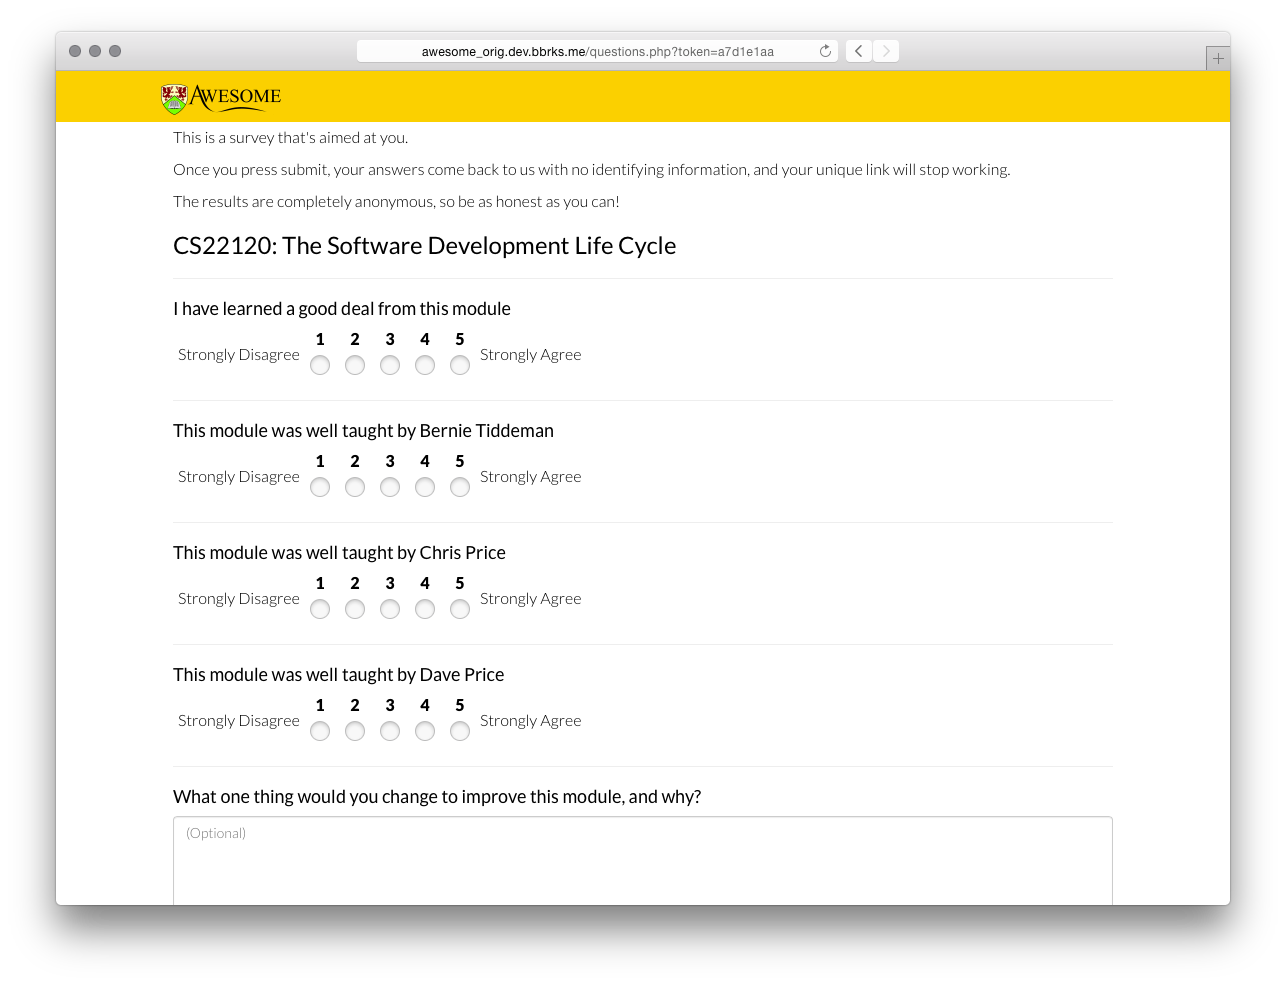
\includegraphics[width=\textwidth]{screens/prototype-questionnaire}
		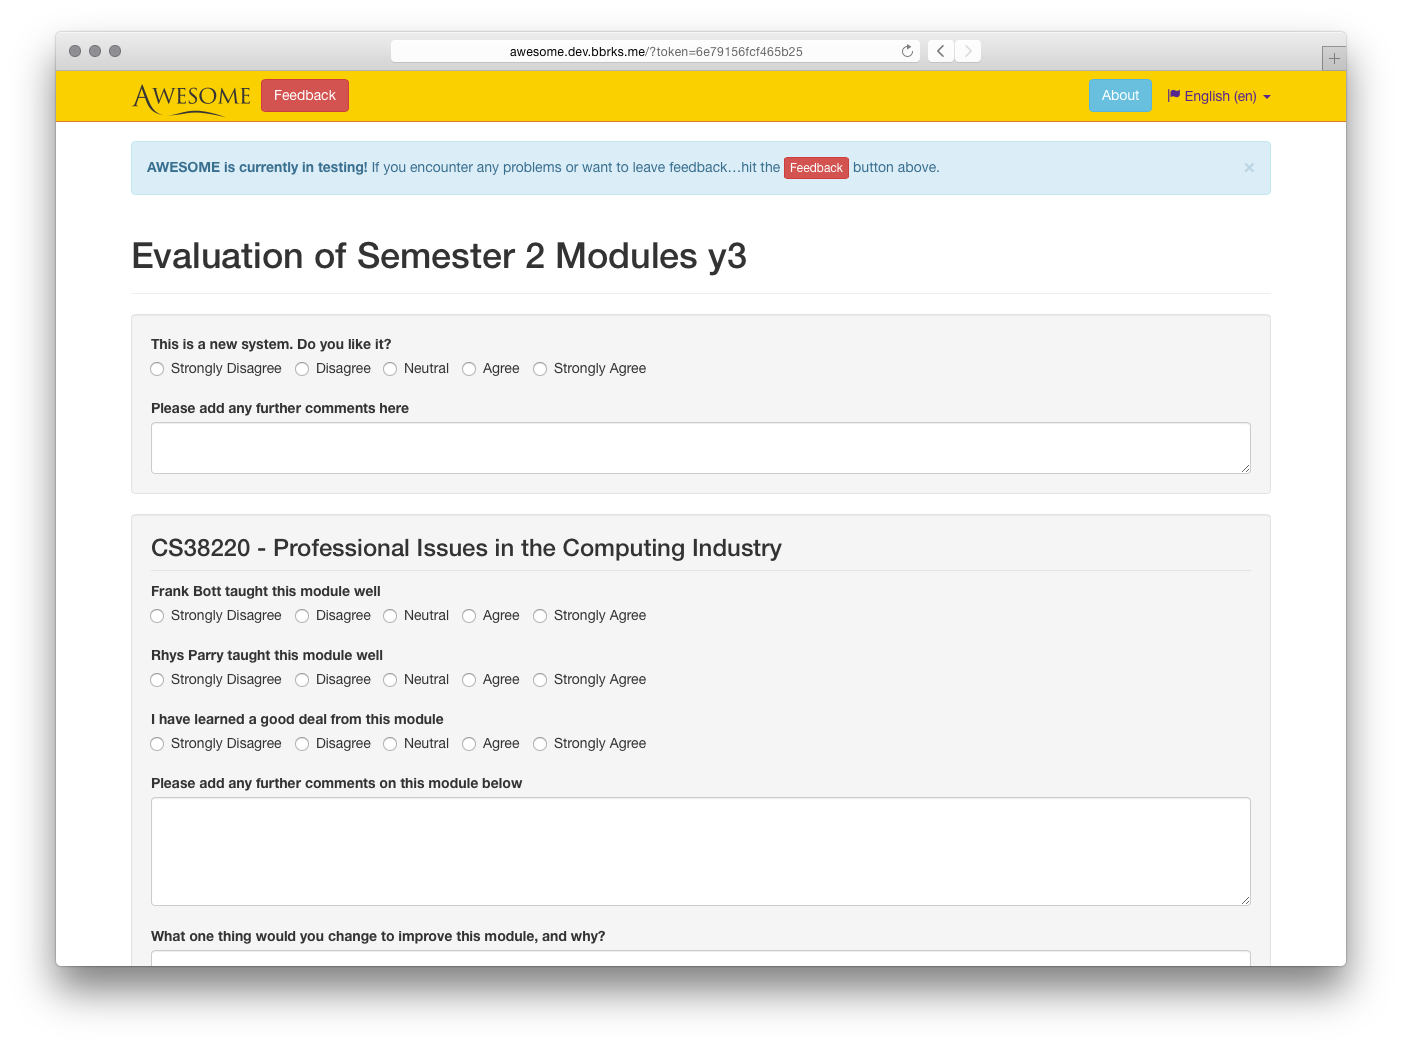
\includegraphics[width=\textwidth]{screens/final-questionnaire}
		\caption{A comparison of questionnaire pages between the prototype version and the submitted version of \acs{AWESOME}}
		\label{fig:questionnaire-comparison}
	\end{figure}
	
	The admin dashboard of the prototype wasn't very user friendly.
	Creating surveys, adding questions, modules, students, and staff was fairly convoluted.
	Results weren't clear to look at, and took up a lot of space per-question by pie charts, which were unnecessary given the data provided.
	
	\begin{figure}[H]
		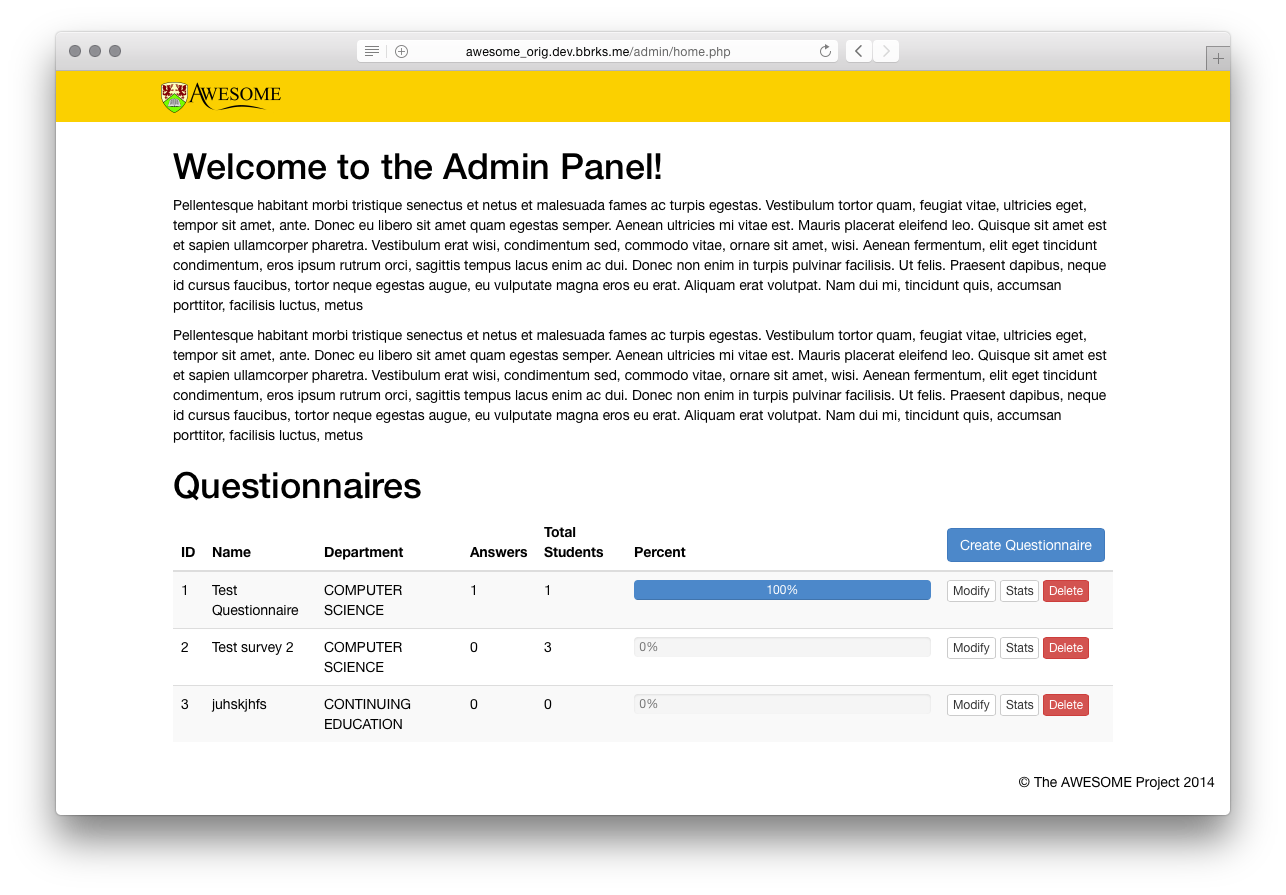
\includegraphics[width=\textwidth]{screens/prototype-viewall}
		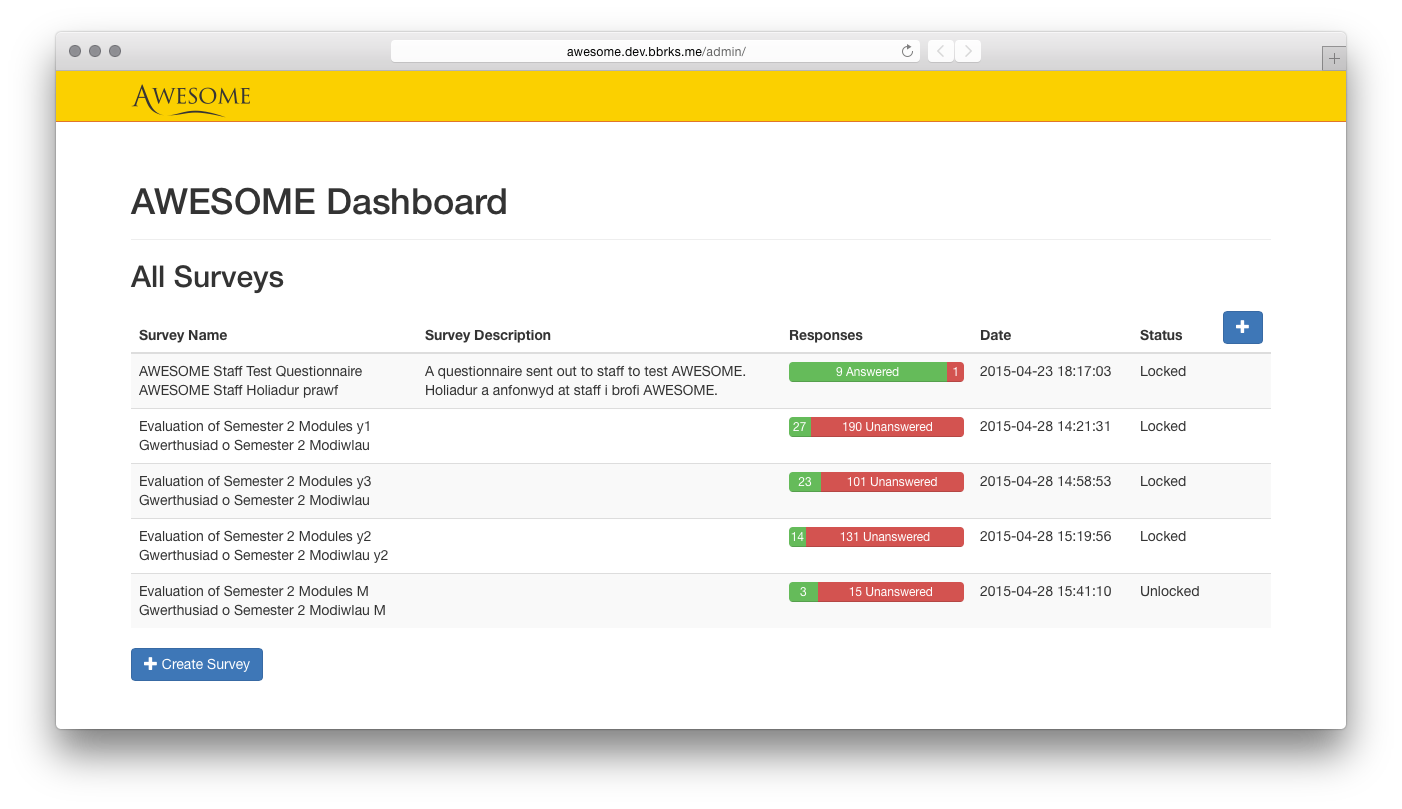
\includegraphics[width=\textwidth]{screens/final-viewall}
		\caption{A comparison of surveys view between the prototype version and the submitted version of \acs{AWESOME}}
		\label{fig:surveys-comparison}
	\end{figure}
	
	\begin{figure}[H]
		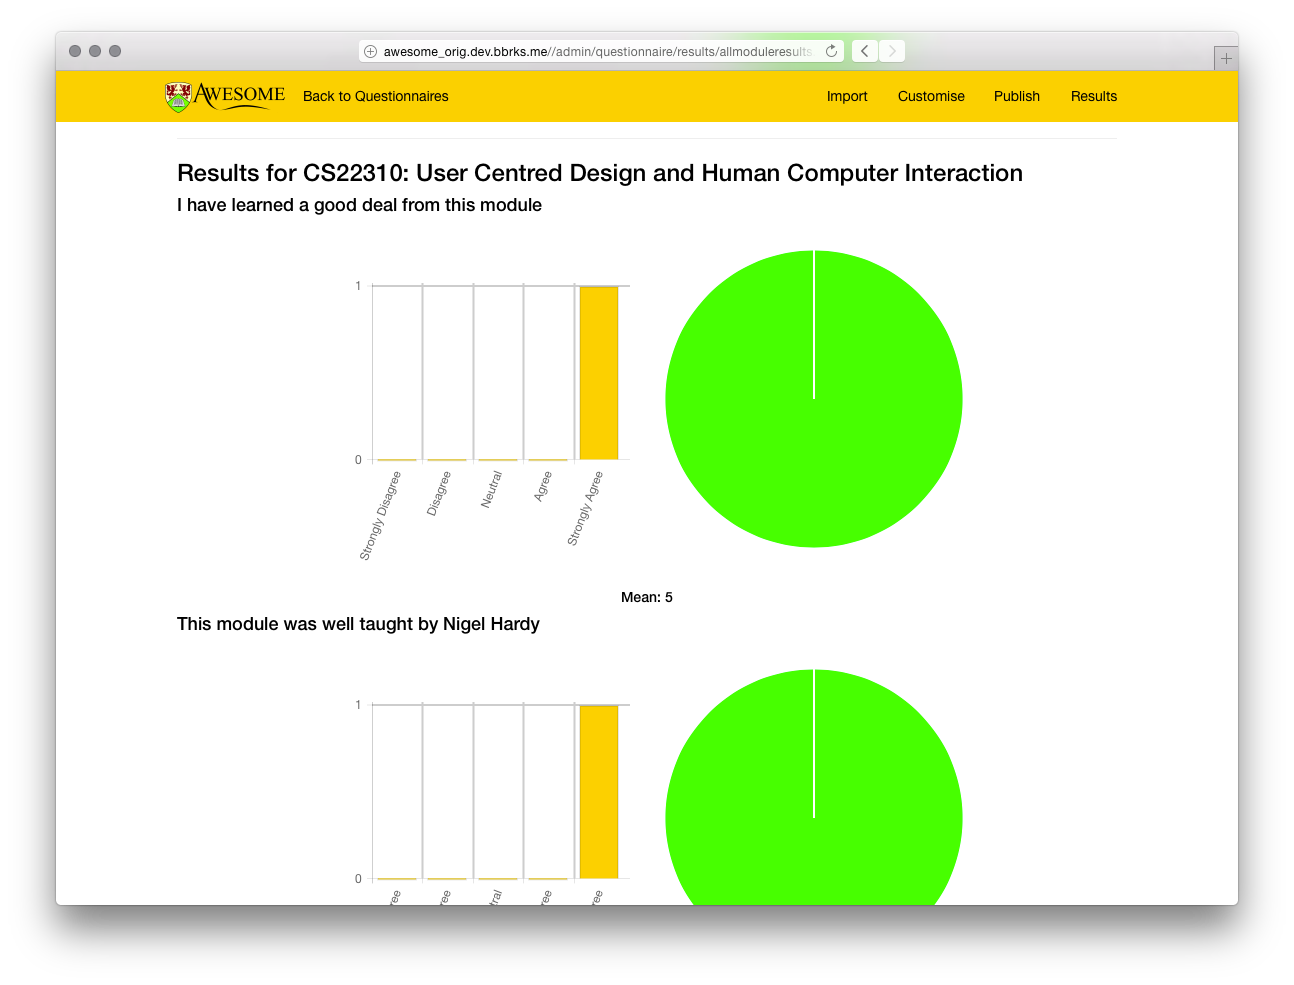
\includegraphics[width=\textwidth]{screens/prototype-results}
		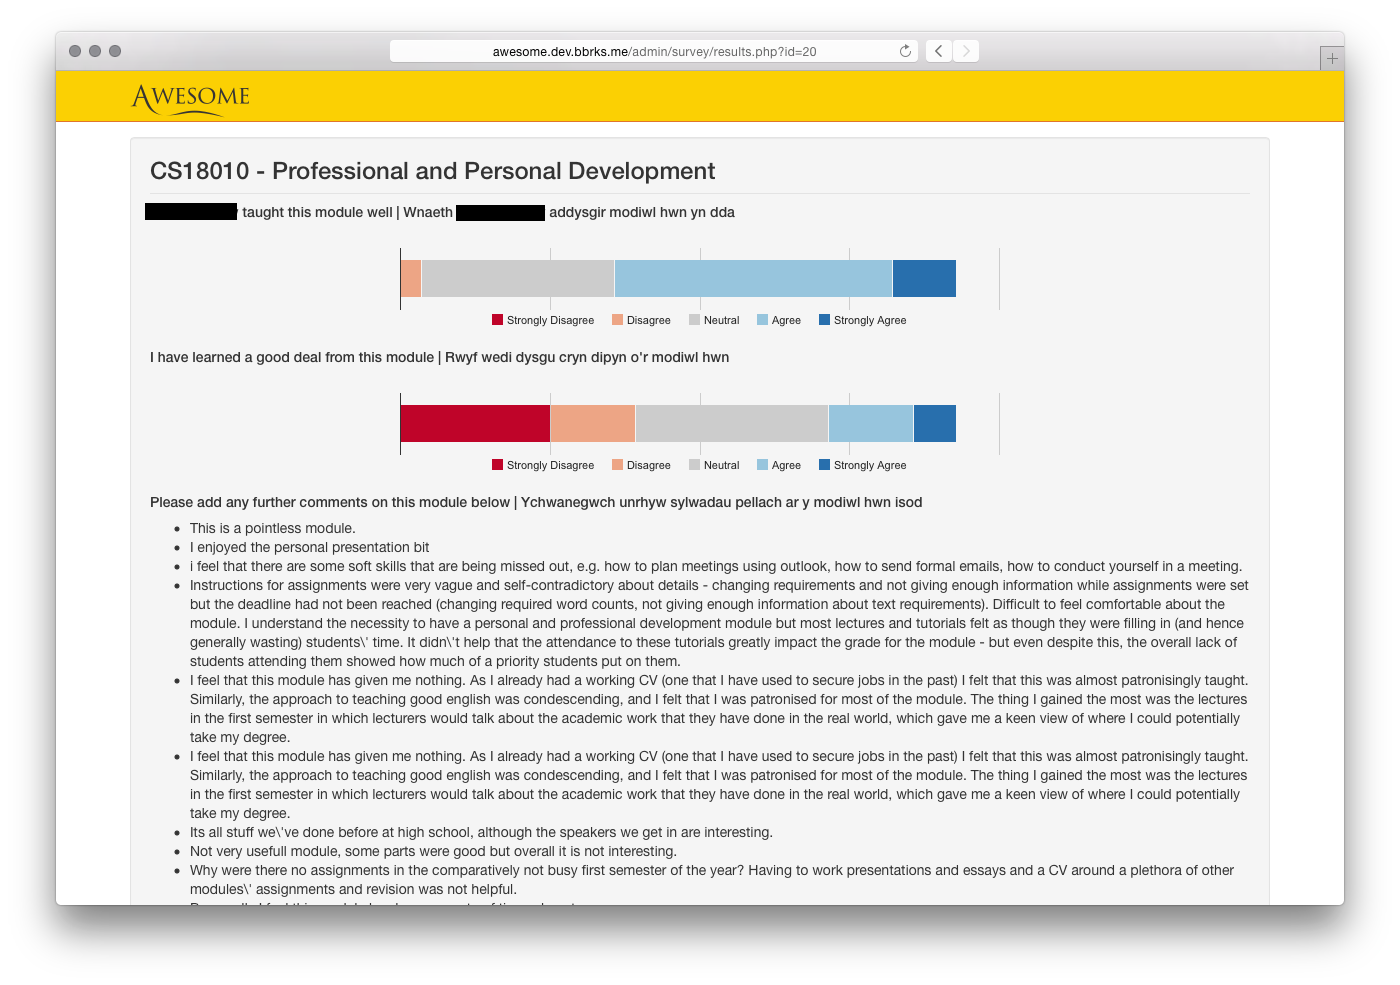
\includegraphics[width=\textwidth]{screens/final-results}
		\caption{A comparison of results between the prototype version and the submitted version of \acs{AWESOME}}
		\label{fig:results-comparison}
	\end{figure}
	
	\begin{figure}[H]
		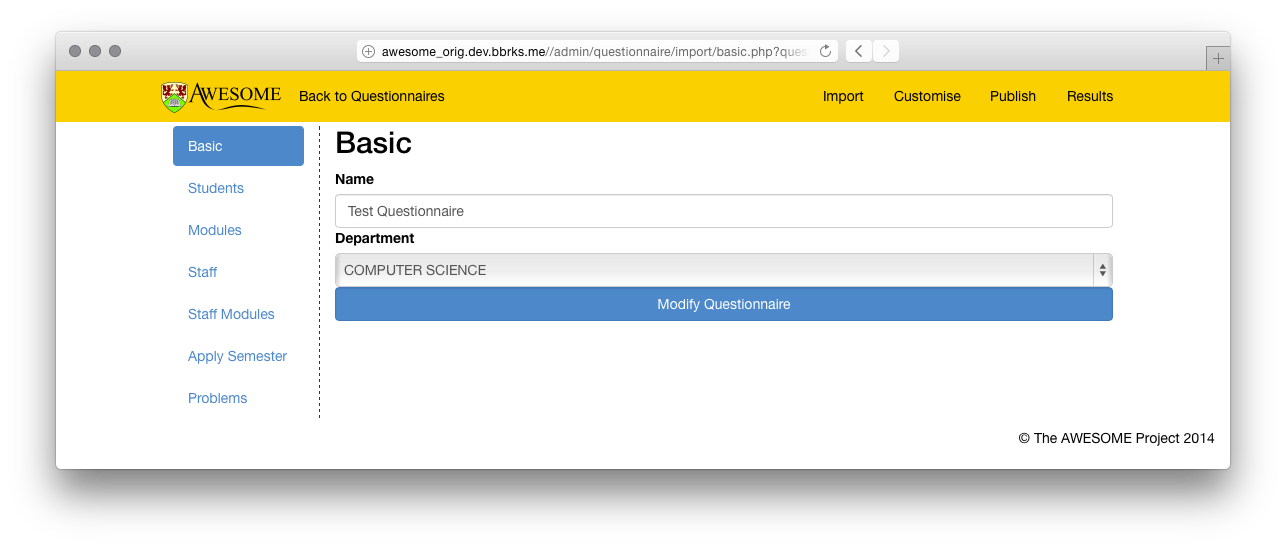
\includegraphics[width=\textwidth]{screens/prototype-single}
		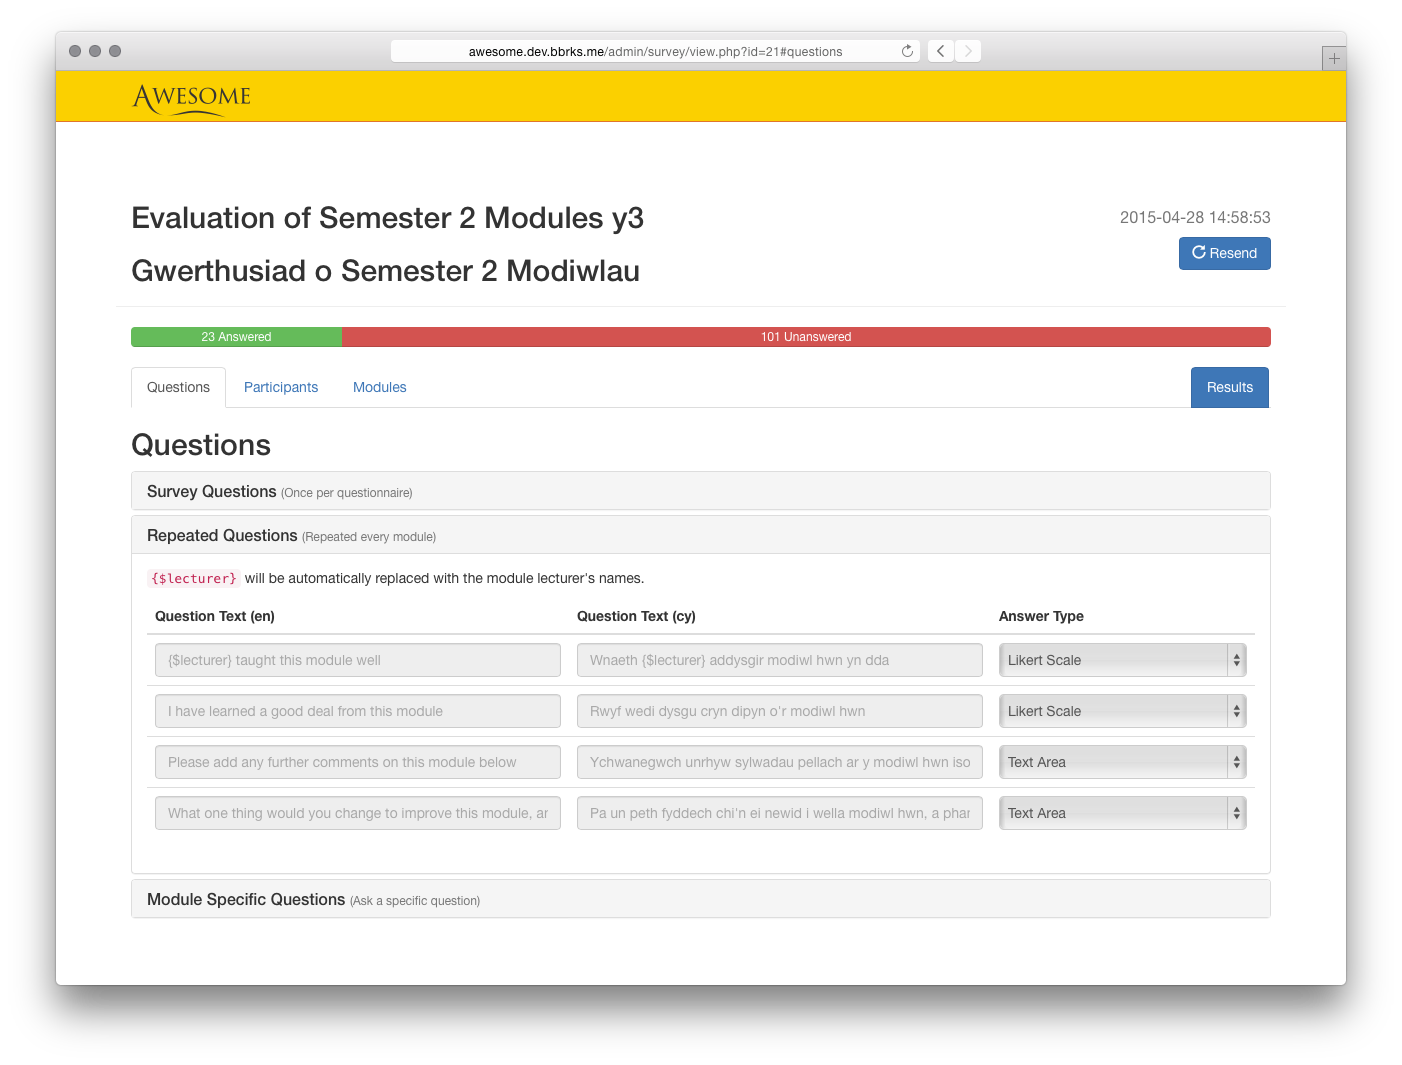
\includegraphics[width=\textwidth]{screens/final-questions}
		\caption{A comparison of survey view between the prototype version and the submitted version of \acs{AWESOME}}
		\label{fig:view-comparison}
	\end{figure}
	
	\begin{figure}[H]
		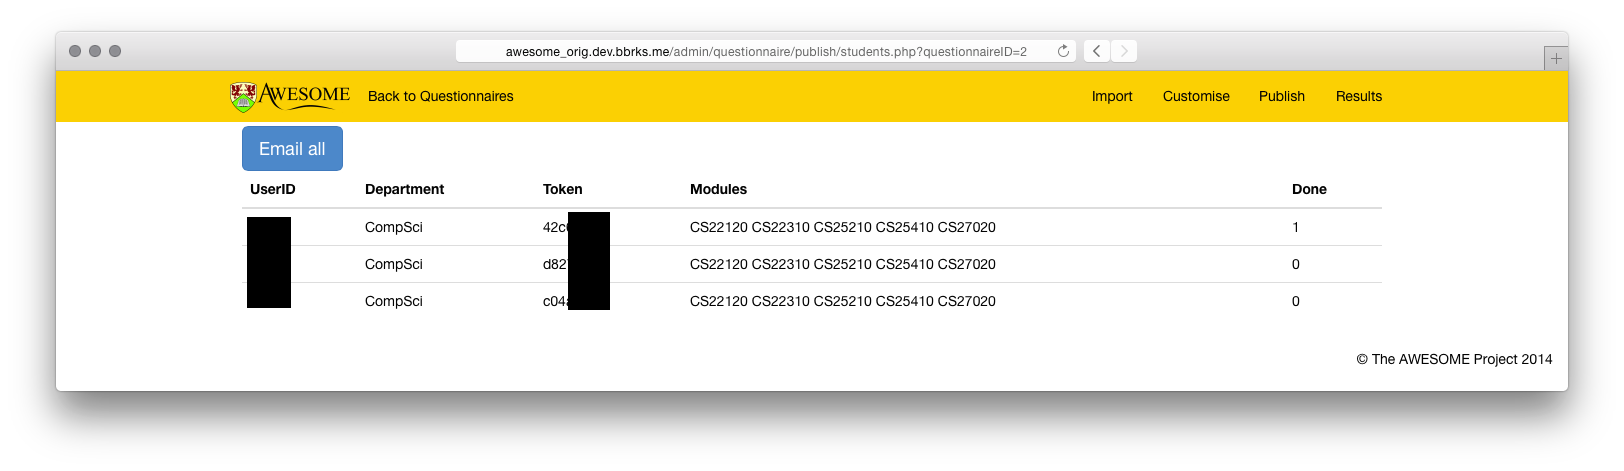
\includegraphics[width=\textwidth]{screens/prototype-respondents}
		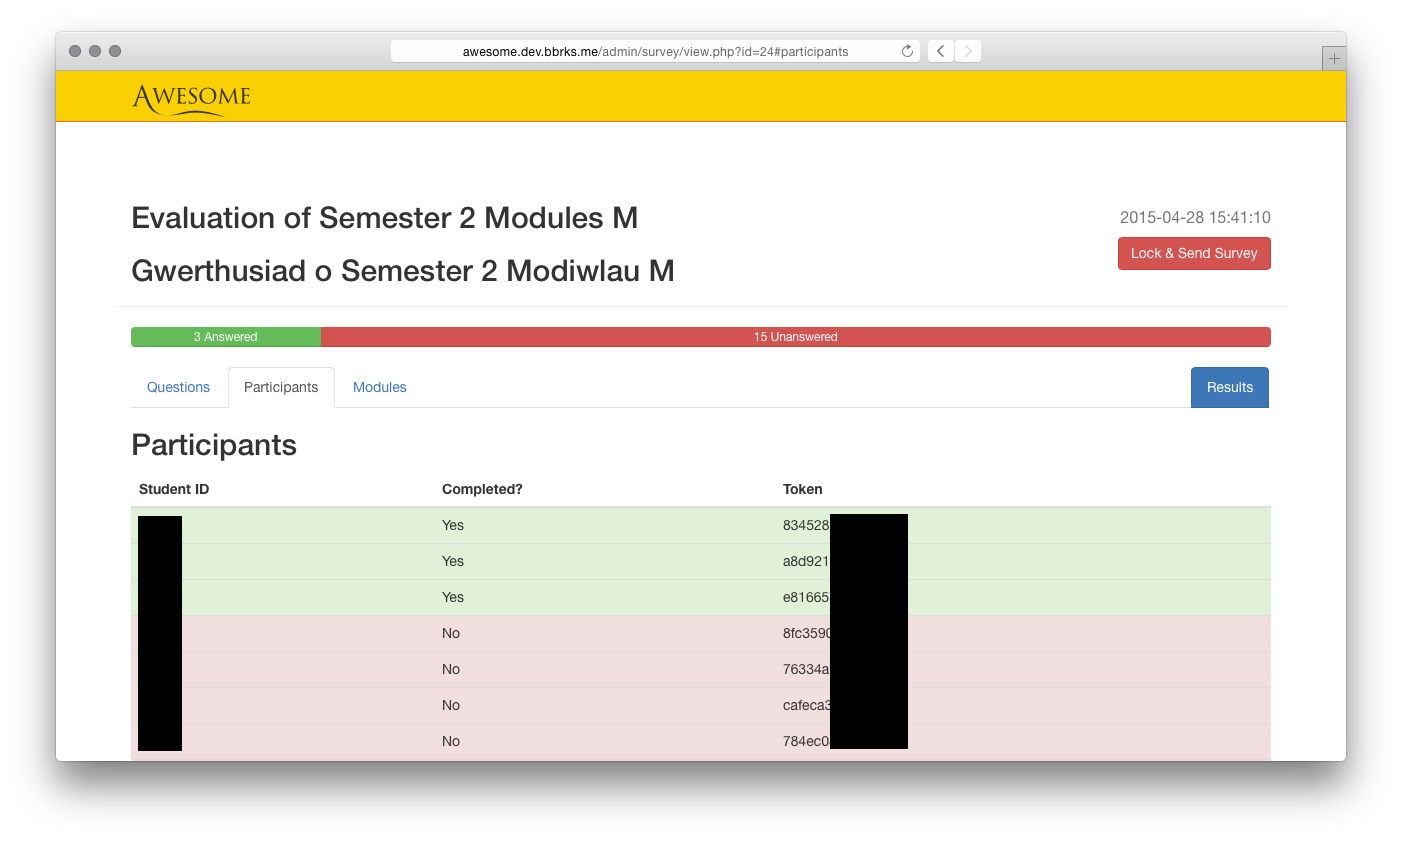
\includegraphics[width=\textwidth]{screens/final-respondents}
		\caption{A comparison of respondents between the prototype version and the submitted version of \acs{AWESOME}}
		\label{fig:respondents-comparison}
	\end{figure}
	
	Additional features include a feedback form when \ac{AWESOME} is in debug mode.
	This allows users to send an email to developers, containing any text they wish, as well as automatically including user-agent and other metadata to help identify the problem.
	
	\begin{figure}[H]
		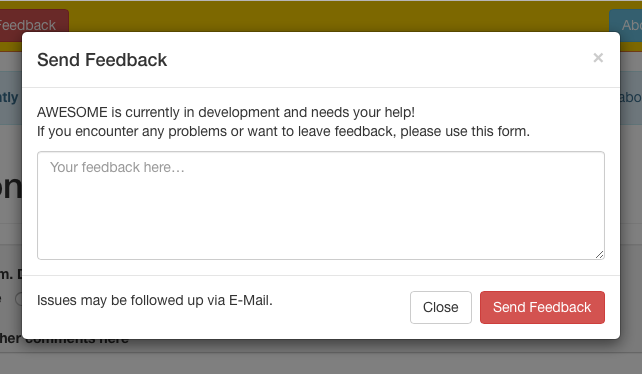
\includegraphics[width=\textwidth]{screens/final-feedbackform}
		\caption{A screenshot of the feedback form in \acs{AWESOME}}
		\label{fig:feedbackform}
	\end{figure}
	